% !TeX program = pdflatex
\documentclass[11pt,a4paper]{article}

% zentrale Einstellungen / Pakete
% ===================== Sprache & Encoding =====================
\usepackage[ngerman]{babel}
\usepackage[T1]{fontenc}
\usepackage[utf8]{inputenc} % für pdfLaTeX
\usepackage{csquotes}
\usepackage{lmodern}
% ===================== Seitenlayout =====================
\usepackage{geometry}
\geometry{top=2cm, bottom=2cm, left=2cm, right=2cm}

% 1,5 Zeilenabstand
\usepackage{setspace}
\onehalfspacing

% Blocksatz-Feintypografie
\usepackage{microtype}

% ===================== Schrift (modern) =====================
\usepackage[sfdefault]{FiraSans} % modern, gut lesbar
\usepackage{FiraMono}           % terminal-artig
\renewcommand{\familydefault}{\sfdefault}

% ===================== Überschriften exakt 12 pt =====================
\usepackage{titlesec}
\titleformat{\section}{\bfseries\fontsize{12pt}{14pt}\selectfont}{\thesection}{1em}{}
\titleformat{\subsection}{\bfseries\fontsize{12pt}{14pt}\selectfont}{\thesubsection}{1em}{}
\titleformat{\subsubsection}{\bfseries\fontsize{12pt}{14pt}\selectfont}{\thesubsubsection}{1em}{}

% Max. 3 Ebenen nummerieren & im ToC zeigen
\setcounter{secnumdepth}{3}
\setcounter{tocdepth}{3}

% Absätze: 6 pt Abstand, kein Erstzeileneinzug
\setlength{\parskip}{6pt}
\setlength{\parindent}{0pt}

% Fußnoten = 10 pt
\makeatletter
\renewcommand\footnotesize{\@setfontsize\footnotesize{10pt}{12pt}}
\makeatother

% ===================== Kopf-/Fußzeile =====================
\usepackage{fancyhdr}
\pagestyle{fancy}
\fancyhf{}
\fancyfoot[C]{\thepage}
\renewcommand{\headrulewidth}{0pt}

% ===================== Grafiken, Tabellen =====================
\usepackage{graphicx}
\usepackage{booktabs}
\usepackage{array}
\usepackage{float}
\usepackage{threeparttable}
\usepackage{tabularx}

% Farben für Tabellen-Zeilen
\usepackage[table]{xcolor} % \rowcolor in Tabellen

% Moderne Tabellen-Box (wie Codeblöcke)
\usepackage[most]{tcolorbox}
\usepackage{tabularray}
\UseTblrLibrary{booktabs}
\tcbuselibrary{listings,breakable}
\newtcolorbox{tableblock}[1][]{
  enhanced,
  breakable,
  colback=black!3,
  colframe=black!12,
  boxrule=0.4pt,
  arc=2mm,
  left=6pt,right=6pt,top=6pt,bottom=6pt,
  #1
}
\renewcommand{\arraystretch}{1.15}
\setlength{\tabcolsep}{6pt}
% Tabelllinien (tabularray) etwas heller
\renewcommand{\lTblrDefaultHruleColorTl}{black!25}
\renewcommand{\lTblrDefaultVruleColorTl}{black!25} % falls du mal vertikale Linien nutzt

% ===================== Code-Blöcke (hellgrau + Terminal-Look) =====================
\usepackage{listings}

\lstdefinestyle{terminal}{
  language=bash,
  basicstyle=\ttfamily\small,
  columns=fullflexible,
  breaklines=true,
  keepspaces=true,
  showstringspaces=false,
  tabsize=2,
  morecomment=[l]{\#},
  commentstyle=\color{green!50!black}\itshape
}

% Umgebung: \begin{codeblock}...\end{codeblock}
\newtcblisting{codeblock}[1][]{
  listing only,
  breakable,
  colback=black!3,
  colframe=black!12,
  boxrule=0.4pt,
  arc=2mm,
  left=6pt,right=6pt,top=6pt,bottom=6pt,
  listing options={style=terminal},
  #1
}

% Inline-Code (optional): \codeinline{...}
\usepackage{xparse}
\NewDocumentCommand{\codeinline}{m}{\texttt{#1}}

% (optional) sauberere Captions (auch für \caption*)
\usepackage[font=small,labelfont=bf]{caption}
% ===================== Hyperlinks (spät laden) =====================
\usepackage[hidelinks]{hyperref}
\usepackage{url}

% ===================== Eigene Verzeichnisse / Registerzuordnung =====================
\usepackage{tocloft}
\usepackage{etoolbox}

% --- Registerzuordnung (Nier-Berlin) -----------------------------
\newlistof{regentry}{rgt}{Registerzuordnung (Nier\,-\,Berlin)}
\newcommand{\listofregister}{\listof{regentry}{Registerzuordnung (Nier\,-\,Berlin)}}
\newcounter{regtab}
\NewDocumentCommand{\RegisterCategory}{O{} m}{%
  \begingroup
  \def\entry{#2}%
  \ifstrempty{#1}{%
    \stepcounter{regtab}%
    \addcontentsline{rgt}{regentry}{Tab \theregtab\quad \entry}%
  }{%
    \addcontentsline{rgt}{regentry}{Tab #1\quad \entry}%
  }%
  \endgroup
}

% ===================== Literatur: biblatex-apa =====================
\usepackage[
  style=apa,
  backend=biber,
  sorting=nyt,
  giveninits=true,
  maxcitenames=2,
  maxbibnames=20,
  doi=true,
  url=true,
  isbn=true
]{biblatex}
\DeclareLanguageMapping{ngerman}{ngerman-apa}
\addbibresource{references.bib}


% ===================== Footnotes in Grau =====================
\usepackage{xcolor}

% Nimm hier deine bestehende Graufarbe oder definiere eine:
\definecolor{FMDGray}{HTML}{6B6B6B} % ggf. anpassen

\makeatletter

% Ziffer (Marker) im Fließtext grau
\renewcommand{\@makefnmark}{%
  \hbox{\textcolor{FMDGray}{\@textsuperscript{\normalfont\@thefnmark}}}%
}

% Fußnotentext + Marker im Fußnotenbereich grau (mit Hanging-Indent)
\renewcommand\@makefntext[1]{%
  \parindent 1em%
  \noindent
  \hb@xt@1.8em{\hss\textcolor{FMDGray}{\@makefnmark}}%
  \textcolor{FMDGray}{#1}%
}

% Fußnoten-Trennlinie grau (kurz + dünn, wie "UI-Linien")
\renewcommand{\footnoterule}{%
  \kern -3pt
  {\color{FMDGray}\hrule width .35\linewidth height .4pt}
  \kern 2.6pt
}
\makeatother


% ------------------ Projektdaten ---------------------------------
\newcommand{\projektname}{FMD Flashcard}
\newcommand{\dokumenttyp}{Projekt-Dokumentation}
\newcommand{\dokumenttitel}{Vault-basierte Lern-App}
\newcommand{\version}{0.1.0}
\newcommand{\status}{Entwurf}
\newcommand{\build}{Commit: \codeinline{<hash>} \quad Branch: \codeinline{main}}
\newcommand{\repo}{\url{https://<dein-repo-link>}}
\newcommand{\autorname}{Marcel Tenhaft}
\newcommand{\kontakt}{\codeinline{<mail>} / \codeinline{<discord/github>}}
\newcommand{\abgabedatum}{Dezember 2025}

% PDF-Metadaten (optional)
\hypersetup{
  pdftitle={\projektname\ - \dokumenttyp},
  pdfauthor={\autorname}
}

\begin{document}

% ======================= TITELSEITEN ==============================
\pagenumbering{Roman}
\thispagestyle{empty}

\begin{titlepage}
  \centering
  {\Large \dokumenttyp \par}
  \vspace{1.2cm}

  {\bfseries\LARGE \projektname \par}
  \vspace{0.3cm}
  {\Large \dokumenttitel \par}

  \vspace{1.8cm}

  \begin{tabular}{@{}ll@{}}
    Version: & \version \\
    Status:  & \status \\
    Datum:   & \abgabedatum \\
    Autor:   & \autorname \\
    Repository: & \repo \\
    Build: & \build \\
    Kontakt: & \kontakt \\
  \end{tabular}

  \vfill
  \small
  Dieses Dokument beschreibt Anforderungen, Architektur, Implementierung und Betrieb des Projekts \projektname.
\end{titlepage}

% ======================= DOKUMENTKONTROLLE ========================
\section*{Änderungshistorie}
\addcontentsline{toc}{section}{Änderungshistorie}

\begin{tabularx}{\textwidth}{@{}l l l X@{}}
\textbf{Version} & \textbf{Datum} & \textbf{Autor} & \textbf{Änderung} \\
\hline
0.1.0 & \abgabedatum & \autorname & Initiale Projektstruktur, Präambel, Kapitel-Imports \\
\end{tabularx}

\newpage

% ======================= VERZEICHNISSE ============================
\tableofcontents
\newpage

\renewcommand{\listfigurename}{Abbildungen}
\renewcommand{\listtablename}{Tabellen}

\begingroup
\setcounter{tocdepth}{0}
\listoffigures
\bigskip
\listoftables
%\listofcommands
\endgroup

\newpage

% ======================= ABKÜRZUNGEN ==============================
\section*{Abkürzungsverzeichnis}
\addcontentsline{toc}{section}{Abkürzungsverzeichnis}

\begin{tabularx}{\textwidth}{@{}llX@{}}
\textbf{Abk.} & \textbf{Deutsch} & \textbf{Englisch / Kommentar} \\
\hline
A/B-Test & Vergleichstest & Split-Run-Test zweier Varianten \\
IT       & Informationstechnologie & Information Technology \\
\end{tabularx}

\newpage

% ======================= HAUPTTEIL ================================
\pagenumbering{arabic}
\setcounter{page}{1}

% Tipp: In deinen Kapiteldateien kannst du Code so setzen:
% \begin{codeblock}[title=Terminal]
% cargo tauri dev
% \end{codeblock}



\begin{figure}[H]
    \centering
    \includegraphics[width=0.35\textwidth]{FMD/image/logo.png}
    \caption{Projektlogo \projektname\ (logo).\cite{Eigendarstellung}}
    \label{fig:zielsetzung-logo}
\end{figure}

\section{Einleitung}
% Was:
Diese Arbeit dokumentiert die Konzeption und Umsetzung des Projekts \projektname, einer Vault-basierten Lern- und Flashcard-Anwendung. Der Schwerpunkt liegt auf der technischen Projektdokumentation (Architektur, Implementierung, Build-/Run-Prozess, Tests und Betrieb), sodass das System nachvollziehbar reproduziert, bewertet und weiterentwickelt werden kann.

% Warum:
Die Dokumentation dient als zentrale Referenz für Entscheidungen und Vorgehensweisen im Projektverlauf. Sie reduziert Einarbeitungszeit, erleichtert Reviews und schafft eine belastbare Grundlage für Wartung, Erweiterungen und spätere Refactorings.

% Ergebnis:
Als Ergebnis entsteht eine strukturierte Projektbeschreibung mit klaren Anforderungen, einem konsistenten Architekturmodell, einem nachvollziehbaren Entwicklungsprozess sowie konkreten Anleitungen für Setup, Nutzung und Betrieb.

\subsection{Motivation}
Digitale Lerninhalte verteilen sich häufig über Notizen, PDFs, Karteikarten-Apps und verschiedene Geräte. Dadurch entstehen Medienbrüche, redundante Inhalte und ein hoher Pflegeaufwand. Insbesondere beim langfristigen Lernen ist es hilfreich, wenn Wissen strukturiert, versionierbar und wiederverwendbar vorliegt.

Das Projekt adressiert dieses Problem durch eine Vault-basierte Organisation der Inhalte (analog zu wissensbasierten Notizsystemen) und verbindet diese mit einer Flashcard-Logik. Ziel ist eine Lösung, die Inhalte konsistent verwaltet, den Lernfortschritt abbildet und gleichzeitig eine einfache Erweiterbarkeit für spätere Funktionen (z.\,B. Synchronisation, Import/Export, Statistiken) ermöglicht.

\subsection{Ziel und Fragestellung}
Ziel des Projekts ist die Entwicklung eines lauffähigen Prototyps einer Lernanwendung, die Lerninhalte in einer klar definierten Datenstruktur (Vault) verwaltet und daraus Flashcards für wiederholtes Lernen ableitet.

Die leitende Fragestellung lautet:
\enquote{Wie kann eine Vault-basierte Lernanwendung so konzipiert und implementiert werden, dass Inhalte reproduzierbar verwaltet, effizient gelernt und technisch wartbar weiterentwickelt werden können?}

\subsection{Beitrag dieses Papers}
Dieses Dokument liefert die für das Projekt wesentlichen Artefakte und Entscheidungen in strukturierter Form:
\begin{itemize}
  \item eine nachvollziehbare Beschreibung der Anforderungen und Zielkriterien,
  \item eine konzeptionelle Architektur (Datenmodell, Komponenten, Schnittstellen),
  \item eine strukturierte Darstellung der Entwicklungsphasen von den Grundlagen bis zum Prototyp,
  \item konkrete Hinweise zu Setup, Build/Run, Konfiguration und Projektstruktur,
  \item eine Zusammenfassung zentraler Entscheidungen, Risiken sowie offener Punkte.
\end{itemize}

\section{Installation \& Entwicklungsumgebung}
Dieses Kapitel beschreibt die notwendigen Voraussetzungen sowie die empfohlene Toolchain, um \projektname lokal zu bauen und auszuführen. Der Schwerpunkt liegt auf einer reproduzierbaren Entwicklungsumgebung und einem klaren Setup-Prozess. Da zentrale Installations- und Diagnoseaufgaben über Skripte automatisiert werden, wird \textbf{Python} als erste Voraussetzung behandelt.









\subsection{Voraussetzungen}
Für die Entwicklung werden folgende Rahmenbedingungen empfohlen:
\begin{itemize}
  \item \textbf{Betriebssystem:} Linux (primär getestet unter Arch Linux).
\item \textbf{Shell/Terminal:} Keine feste Shell-Vorgabe. Die Projektsteuerung erfolgt über  \textbf{Python-Skripte}; eine interaktive Shell wird lediglich zum Aufruf der Befehle benötigt.
  \item \textbf{Zugriffsrechte:} Installation von Paketen/Toolchains (je nach System via Paketmanager).
  \item \textbf{Versionsverwaltung:} Git.
\end{itemize}

\subsubsection{Layer-Modell der Entwicklungsumgebung}

Zur besseren Einordnung der eingesetzten Werkzeuge lässt sich die Entwicklungsumgebung in funktionale Layer gliedern. Diese Layer beschreiben nicht die Programmarchitektur, sondern die Umgebung, in der Entwicklung, Build und Ausführung stattfinden.

\begin{itemize}
  \item \textbf{Basissystem (System Layer)} \\
  Betriebssystem und grundlegende Systemdienste (Linux, macOS, Windows) bilden die technische Basis. In diesem Layer befinden sich außerdem systemweite Werkzeuge wie Git, Compiler, Paketmanager und Laufzeitumgebungen.

  \item \textbf{Automatisierungs- und Skript-Layer} \\
  Installations-, Diagnose- und Steuerungslogik ist plattformübergreifend in \textbf{Python} implementiert. Dieser Layer kapselt wiederkehrende Aufgaben wie Setup, Dependency-Prüfung, Build und Start des Projekts und abstrahiert Plattformunterschiede.

  \item \textbf{Tool- und Framework-Layer} \\
  Entwicklungswerkzeuge und Frameworks wie Rust, Node.js, Tauri sowie der verwendete Paketmanager stellen die eigentliche Build- und Laufzeitumgebung für Backend und Frontend bereit.

  \item \textbf{Entwicklungs- und Prozess-Layer} \\
  IDEs (z.\,B. VS Code), Editor-Erweiterungen, Linter, Formatter und Dev-Server unterstützen den täglichen Entwicklungsprozess. Dieser Layer beeinflusst die Developer Experience, jedoch nicht das resultierende Programmverhalten.
\end{itemize}

Dieses Layer-Modell dient der strukturellen Einordnung der Entwicklungsumgebung und schafft eine klare Trennung zwischen Systembasis, Automatisierung, Toolchain und entwicklungsbegleitenden Prozessen.


\begin{figure}[H]
    \centering
    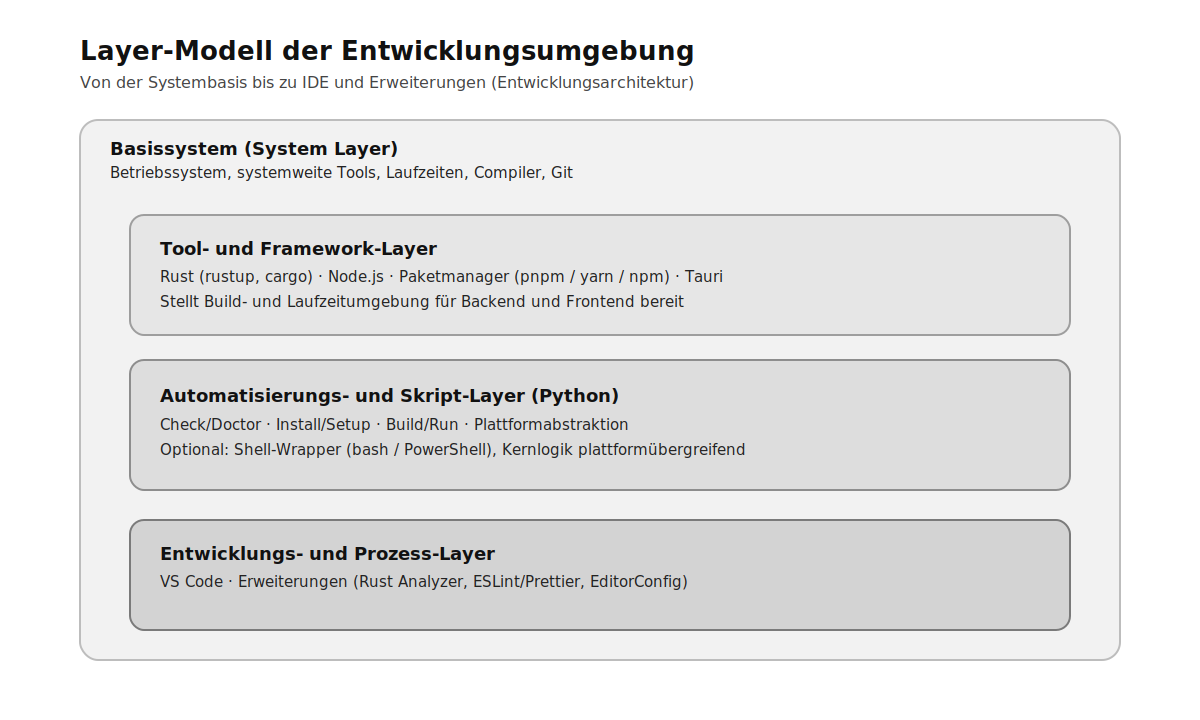
\includegraphics[width=0.95\textwidth]{FMD/image/LayerDevelopDE.png}
    \caption{Layer-Modell \projektname\ .\cite{Eigendarstellung}}
    \label{fig:zielsetzung-architektur}
\end{figure}


\subsection{Voraussetzung: Python}
Python ist eine weit verbreitete, plattformübergreifende Programmiersprache, die häufig für Automatisierung, Systemadministration und Tooling eingesetzt wird. In diesem Projekt wird Python primär als \textbf{administrative Unterstützung} genutzt: Installations- und Setup-Schritte werden über Skripte standardisiert, und das Checkup-/Diagnose-Skript verwendet Python, um Systemzustand, Abhängigkeiten und Toolchain konsistent zu prüfen.\cite{python:official}\footnote{\url{https://www.python.org/}}

\textbf{Warum Python zuerst?}
\begin{itemize}
  \item Installationsskripte und Checks können damit auf \textbf{Windows, Linux und macOS} einheitlich ausgeführt werden.
  \item Python eignet sich für robuste Systemabfragen (z.\,B. Pfade, Versionen, verfügbare Tools) und reduziert manuelle Fehler.
  \item Das Projekt nutzt Python nicht als Laufzeitabhängigkeit der Anwendung selbst, sondern als \textbf{Tooling-Schicht} rund um Setup und Wartung.
\end{itemize}

\textbf{Hinweis zur Vorinstallation:}
Auf vielen Linux-Distributionen ist \codeinline{python3} in typischen Desktop-Installationen bereits vorhanden (z.\,B. Ubuntu, Fedora Workstation, openSUSE Leap).
Das ist jedoch nicht garantiert: Bei Minimal-Images oder sehr schlanken Installationen kann Python fehlen (z.\,B. bei einer reinen Arch-\codeinline{base}-Installation).
Auf macOS wird Python nicht zuverlässig mitgeliefert und sollte daher explizit installiert werden.
Für eine reproduzierbare Umgebung wird in jedem Fall empfohlen, die verwendete Python-Version zu prüfen und zu dokumentieren.

\textbf{Beispiel Installationsbefehle:}

\begin{codeblock}[title=Python installieren (Beispiele)]

#  Arch Linux (Details vollstaendiges Setup: siehe Anhang A)
sudo pacman -S python python-pip

# Fedora / RPM-basiert (DNF)
sudo dnf install -y python3 python3-pip

# Ubuntu/Debian
sudo apt update
sudo apt install python3 python3-pip

# macOS (Homebrew)
brew install python

# Windows (Winget)
winget install -e --id Python.Python.3
\end{codeblock}

\subsubsection{Prüfen der Installation}
Nach der Installation sollte die Python-Version überprüft werden. Je nach System ist Python entweder über \codeinline{python} oder \codeinline{python3} erreichbar.

\begin{codeblock}[title=Python-Version prüfen]
python3 --version
# alternativ (falls passend):
python --version
\end{codeblock}
\subsection{Voraussetzung: Git}
Git ist ein verteiltes Versionsverwaltungssystem, das Änderungen am Quellcode nachvollziehbar speichert und Zusammenarbeit über Branches, Commits und Tags ermöglicht. In diesem Projekt wird Git benötigt, um das Repository zu klonen, Updates einzuspielen und Stände reproduzierbar zu referenzieren (z.\,B. über Tags/Commits).

\textbf{Warum Git?}
\begin{itemize}
  \item \textbf{Reproduzierbarkeit:} definierte Stände über Tags/Commits
  \item \textbf{Nachvollziehbarkeit:} Historie von Änderungen und Entscheidungen
  \item \textbf{Zusammenarbeit:} Branching/Merging für parallele Entwicklung
\end{itemize}

\textbf{Hinweis zur Vorinstallation:}
Ob Git bereits vorinstalliert ist, hängt vom Betriebssystem und der jeweiligen Installation (Desktop vs. Minimal-Image) ab.
Auf macOS ist Git häufig über die Xcode Command Line Tools verfügbar bzw. wird beim ersten Aufruf nachinstalliert. Auf einigen Linux-Images kann Git bereits vorhanden sein (z.\,B. wird es bei Fedora Silverblue häufig mitgeliefert), bei Minimalinstallationen ist es jedoch nicht garantiert.

Praxisbeispiel: In der Testumgebung (Arch Linux / CachyOS) waren Git und Python bereits vorinstalliert; dies kann je nach Distribution und Installationsprofil abweichen.

\textbf{Beispiel Installationsbefehle:}

\begin{codeblock}[title=Git installieren (Beispiele)]
# Arch Linux
sudo pacman -S git

# Fedora / RPM-basiert
sudo dnf install git-all

# Ubuntu/Debian
sudo apt update
sudo apt install git

# macOS (Apple/Xcode CLT oder Homebrew)
xcode-select --install
# alternativ:
brew install git

# Windows (Winget)
winget install --id Git.Git -e --source winget
\end{codeblock}

\subsubsection{Prüfen der Installation}
Nach der Installation sollte Git verfügbar sein:

\begin{codeblock}[title=Git-Version prüfen]
git --version
\end{codeblock}
\subsection{Quickstart}
Die folgenden Schritte zeigen den schnellsten Weg, um \projektname lokal zu starten. Das Setup wird über das Control-/Checkup-Tooling standardisiert (z.\,B. \codeinline{doctor}, \codeinline{install}, \codeinline{run}). 

\begin{codeblock}[title={Quickstart: Clone the repo \& switch to a standard project directory}]
# Standard project directory (works on Linux systems):
mkdir -p ~/Projects
cd ~/Projects

# Clone repository (replace URL)
git clone https://github.com/kleiveist/FMDFlashcard.git
cd FMDFlashcard

# Control-Skript
cd ~/Projects/FMDFlashcard
# optional: health check / doctor
python3 tools/control.py --doctor

# Install & start
cd ~/Projects/FMDFlashcard
python3 tools/control.py --install
\end{codeblock}


\textit{Hinweis:} Das Beispiel oben zeigt die Befehle für ein Linux-System; unter macOS sind \texttt{git clone} und \texttt{cd} identisch. Unter Windows funktionieren die Befehle in \enquote{Git Bash} wie unter Linux; in PowerShell/CMD ebenfalls, nur das Auflisten des Verzeichnisses erfolgt typischerweise mit \texttt{dir} (PowerShell unterstützt auch \texttt{ls}).

Nach dem Ausführen von \texttt{python3 tools/control.py --doctor} wird eine Auflistung der noch fehlenden Pakete und Module angezeigt. Diese werden anschließend automatisch mit folgendem Befehl installiert:

\begin{verbatim}
python3 tools/control.py --install
\end{verbatim}

Nach der Installation wird \texttt{python3 tools/control.py --doctor} erneut ausgeführt. Das Ergebnis ist in Abbildung~\ref{fig:terminal-checkup} dargestellt.

\begin{figure}[H]
    \centering
    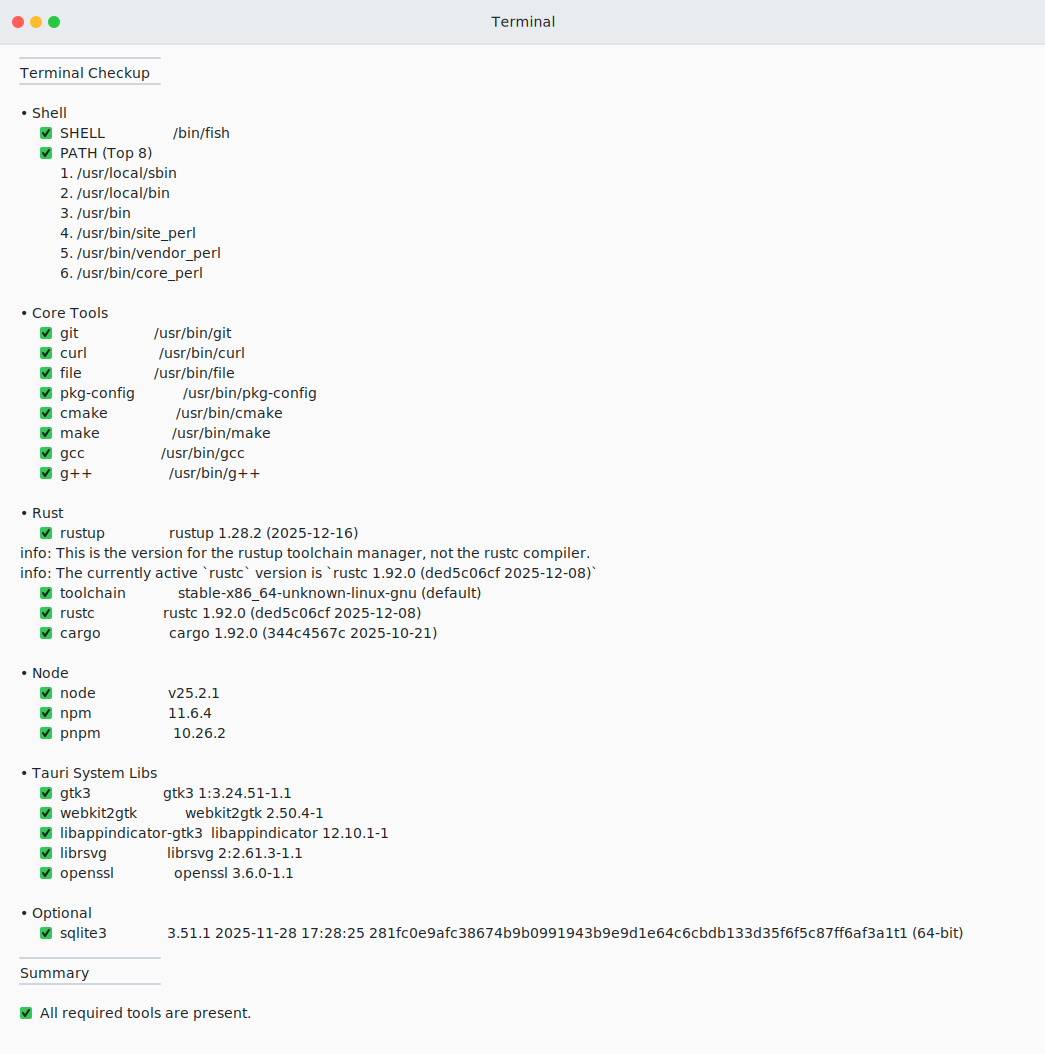
\includegraphics[width=0.9\textwidth]{FMD/image/terminal_checkup_light.png}
    \caption{Terminal Checkup.\cite{Eigendarstellung}}
    \label{fig:terminal-checkup}
\end{figure}



\subsubsection{Terminal Checkup}
In den folgenden Unterabschnitten werden die einzelnen Bereiche der Terminal-Überprüfung erläutert. Ziel ist es, die angezeigten Komponenten kurz einzuordnen und zu begründen, warum diese Prüfungen durchgeführt werden. Dadurch wird sichergestellt, dass alle notwendigen Werkzeuge und Systemabhängigkeiten für Installation, Build und Ausführung der Anwendung vorhanden und korrekt konfiguriert sind.

\subsection{Erläuterung der Checkup-Bereiche}
Die folgenden Punkte erklären die im Terminal-Checkup ausgegebenen Bereiche und deren Zweck.

\begin{itemize}
    \item \textbf{Shell (in den meisten Systemen bereits installiert):}
    Zeigt die verwendete Shell sowie die \texttt{PATH}-Konfiguration. Damit wird geprüft, ob wichtige Programme über die Kommandozeile gefunden werden und die Entwicklungsumgebung korrekt eingerichtet ist.

    \item \textbf{Core Tools (in den meisten Systemen bereits installiert):}
    Enthält grundlegende Entwicklungswerkzeuge (z.\,B. \texttt{git}, Compiler, Build-Tools). Diese werden benötigt, um Quellcode zu beziehen, native Abhängigkeiten zu kompilieren und Build-Prozesse zuverlässig auszuführen.

    \item \textbf{Rust:}
    Prüft die Rust-Toolchain (\texttt{rustup}, \texttt{rustc}, \texttt{cargo}). Dies ist erforderlich, da das Tauri-Backend in Rust gebaut wird und ohne eine passende Toolchain keine Kompilierung und kein Packaging möglich ist.

    \item \textbf{Node:}
    Überprüft Node.js sowie Paketmanager wie \texttt{npm}/\texttt{pnpm}. Diese werden für das Frontend benötigt, um JavaScript-Abhängigkeiten zu installieren und das Web-Bundle für die Tauri-App zu erstellen.

    \item \textbf{Tauri System Libs:}
    Listet systemweite Bibliotheken auf, die unter Linux für WebView und GUI-Funktionalitäten notwendig sind (z.\,B. \texttt{gtk3}, \texttt{webkit2gtk}, \texttt{openssl}). Dadurch wird sichergestellt, dass die Anwendung sowohl gebaut als auch zur Laufzeit korrekt ausgeführt werden kann.
\end{itemize}

\paragraph{Hinweis zu Windows und macOS}
Neben der Linux/Unix-Variante existieren auch Installationsskripte für Windows und macOS, die über die automatische Betriebssystem-Erkennung in \texttt{control.py} referenziert werden (u.\,a. \texttt{installwin.py} und \texttt{installmac.py}). :contentReference[oaicite:0]{index=0}
Diese Skripte sind derzeit jedoch noch nicht in virtuellen Maschinen (VMs) verifiziert bzw. reproduzierbar erprobt worden und gelten deshalb als \textit{ungetestet}. 

\subsection{Toolchain und Frameworks}
Tabelle~\ref{tab:toolchain} fasst die eingesetzten Werkzeuge zusammen. Versionen sind als Mindestempfehlung zu verstehen und können projektabhängig angepasst werden (z.\,B. via \codeinline{.tool-versions}, \codeinline{rust-toolchain.toml} oder \codeinline{package.json}).

\begin{table}[H]
\centering
\begin{tblr}{
  colspec = {Q[l,wd=0.28\textwidth] Q[c,wd=0.18\textwidth] Q[l,wd=0.54\textwidth]},
  row{1} = {font=\bfseries, bg=black!6},
  row{even} = {bg=black!2},
  rowsep = 4pt,
  leftsep = 6pt,
  rightsep = 6pt
}
\toprule
Tool/Framework & Version & Zweck im Projekt \\
\midrule
Git & >= 2.x & Repository klonen, Branching, Versionsverwaltung \\
VS Code & aktuell & IDE/Editor; empfohlen für konsistente Formatierung und Debugging \\
Rust (rustup, cargo) & >= 1.7x & Backend/Build (abhängig vom Projektanteil in Rust) \\
Node.js & >= 18 LTS & Frontend/Tooling (Build, Dev-Server, Bundling) \\
Paketmanager (pnpm/yarn/npm) & projektspezifisch & Abhängigkeiten installieren, Scripts ausführen \\
Control-Skript (\codeinline{control.sh}) & repo-intern & Standardisierte Befehle: Check, Install, Build, Run \\
\bottomrule
\end{tblr}
\caption{Toolchain-Übersicht}
\label{tab:toolchain}
\end{table}





\subsubsection{Empfohlene VS-Code-Erweiterungen}
Für eine konsistente Developer Experience werden folgende Erweiterungen empfohlen (optional):
\begin{itemize}
  \item \textbf{Rust Analyzer} (Rust-IDE-Features)
  \item \textbf{EditorConfig} (einheitliche Formatierung)
  \item \textbf{ESLint} / \textbf{Prettier} (bei JavaScript/TypeScript-Frontend)
\end{itemize}

\subsection{Setup-Schritte}
Dieser Abschnitt beschreibt die grundlegenden Setup-Schritte unabhängig vom Betriebssystem. OS-spezifische Installationsbefehle sind im Anhang dokumentiert.

\subsubsection{Repository beziehen}
\begin{codeblock}[title=Repository klonen]
git clone <REPO-URL>
cd <PROJEKT-ORDNER>
\end{codeblock}

\subsubsection{Abhängigkeiten installieren}
Wenn das Projekt ein Control-Skript bereitstellt, sollte dieses bevorzugt genutzt werden, da es wiederholbare Abläufe kapselt.

\begin{codeblock}[title=Installation via Control-Skript]
./control.sh doctor
./control.sh install
\end{codeblock}

Alternativ können (je nach Projektstruktur) die Abhängigkeiten direkt über den jeweiligen Paketmanager bzw. Cargo installiert werden:

\begin{codeblock}[title=Installation ohne Control-Skript (Beispiel)]
# Frontend
pnpm install

# Rust-Anteile (falls erforderlich)
cargo fetch
\end{codeblock}

\subsubsection{Projekt starten (Entwicklung)}
\begin{codeblock}[title=Start (Dev)]
./control.sh run
\end{codeblock}

\subsection{Arch Linux: OS-spezifische Installation (Anhang)}
Die vollständige Installationsanleitung für Arch Linux inklusive systemabhängiger Pakete und dem vollständigen Setup-Skript ist im Anhang dokumentiert:
\begin{itemize}
  \item \textbf{Anhang~A:} Installationsskript und Paketliste für Arch Linux
\end{itemize}

Für weitere Betriebssysteme (z.\,B. Ubuntu/Debian, Fedora, Windows, macOS) kann die Anleitung analog ergänzt werden. Dabei ist insbesondere auf systemabhängige Bibliotheken und Build-Tools zu achten (Compiler, Linker, ggf. UI-Framework-Abhängigkeiten).

\section{Diskussion und Ausblick}
% Zweck: Einordnen, Grenzen und Zukunft aufzeigen

\subsection{Limitationen des Ansatzes}
% Was:
% - Vereinfachungen in der Simulation (Physik, Grafik, Komplexität der NPC-Psychologie)
% - Grenzen lokaler Modelle (Kontextfenster, Qualität der Entscheidungen)
% - Technische Grenzen (Hardware, Entwicklungszeit)
% Warum:
% - Ehrlicher Blick auf Schwächen und offene Punkte

\subsection{Zukünftige Arbeiten}
% Was:
% - Ausbau der NPC-Persönlichkeiten und Langzeitgedächtnisse
% - Nutzung größerer oder spezialisierter Modelle
% - Integration realer AI-Karten, falls verfügbar
% - Ausbau des Projekts als Standard-Benchmark für die Industrie
% Warum:
% - Zeigen, dass das Konzept skalierbar und weiterentwickelbar ist

\section{Fazit}
% Was:
% - Kurze Zusammenfassung der Vision: LifeLLM als Life-Sim-LLM-System und Hardware-Benchmark
% - Wichtigste Punkte: Ereignisgraph, NPC-Massen, LLM-gesteuerte Ereignisse, Hardware-Argument
% - Abschließende Aussage, warum dieses Projekt eine sinnvolle Richtung für Gaming + KI + Hardware ist


% ======================= LITERATUR ================================
\clearpage
\printbibliography[heading=bibintoc, title={Literaturverzeichnis}]
\clearpage

% ======================= ANHANG ===================================
\section*{Verzeichnis der Anhänge}
\addcontentsline{toc}{section}{Verzeichnis der Anhänge}

\appendix
\section{Beispielanhänge}

\end{document}
